\chapter*{Présentation de l'INSI}

\begin{enumerate}
	\def\labelenumi{\arabic{enumi}.}
	\item
	\textbf{Information d'ordre général}
\end{enumerate}
INSI (Institut National Supérieur d'Informatique) est un institut
universitaire situé à Antananarivo, spécialisé dans le domaine de
l'informatique. Il accueille principalement des bacheliers ayant choisi
cette filière, mais reste également ouvert à toute personne manifestant
un intérêt particulier pour les métiers du numérique, à travers son
centre de formation professionnelle.

L'établissement a été fondé le 17 août 2021 et son siège se
trouve à Ankazotokana Ambanidia, Lot VF 32 Ter.

Pour tout renseignement, vous pouvez nous contacter par email à
contact@insi.mg ou visiter notre site web :
\href{http://www.insi.mg/}{www.insi.mg}

INSI University bénéficie du soutien d'entreprises partenaires, dont
Ilo Madagascar SARLU et Data Pulse Center, qui sont
également à l'origine de sa création.

\begin{enumerate}
	\def\labelenumi{\arabic{enumi}.}
	\setcounter{enumi}{1}
	\item
	\textbf{Missions et historiques}
\end{enumerate}

INSI University a été fondée le 17 août 2021 à Antananarivo,
dans un contexte marqué par une forte demande de compétences dans le
domaine de l'informatique et des technologies numériques,

Créé à l'initiative de Ilo Madagascar SARLU} et Data
	Pulse Center, l'Institut a vu le jour avec pour ambition de former une
nouvelle génération de professionnels qualifiés, capables de répondre
aux besoins du marché local et international.

Depuis sa création, INSI ne cesse d'évoluer en adaptant ses formations
aux enjeux technologiques actuels, tout en favorisant un apprentissage
pratique, orienté vers les réalités du monde professionnel.

La mission principale de l'INSI est de former des experts
	compétents, éthiques et innovants dans le domaine de l'informatique,
capables de contribuer activement au développement économique et
numérique de Madagascar.

L'Institut s'engage à :

\begin{itemize}
	\item
	Offrir des formations de qualité, à jour des évolutions
	technologiques,
	\item
	Favoriser l'insertion professionnelle de ses apprenants,
	\item
	Créer un lien fort entre la formation académique et les besoins réels
	des entreprises,
	\item
	Encourager l'entrepreneuriat et l'innovation technologique,
	\item
	Contribuer à la démocratisation de l'accès au savoir numérique.
	
	\begin{enumerate}
		\def\labelenumi{\arabic{enumi}.}
		\item
		\textbf{Organigramme de l'INSI}
	\end{enumerate}
\end{itemize}

L'organigramme ci-dessous présente la structure organisationnelle de
l'INSI, mettant en évidence les différentes fonctions et responsabilités
au sein de l'institut, ainsi que les liens hiérarchiques entre les
divers services.

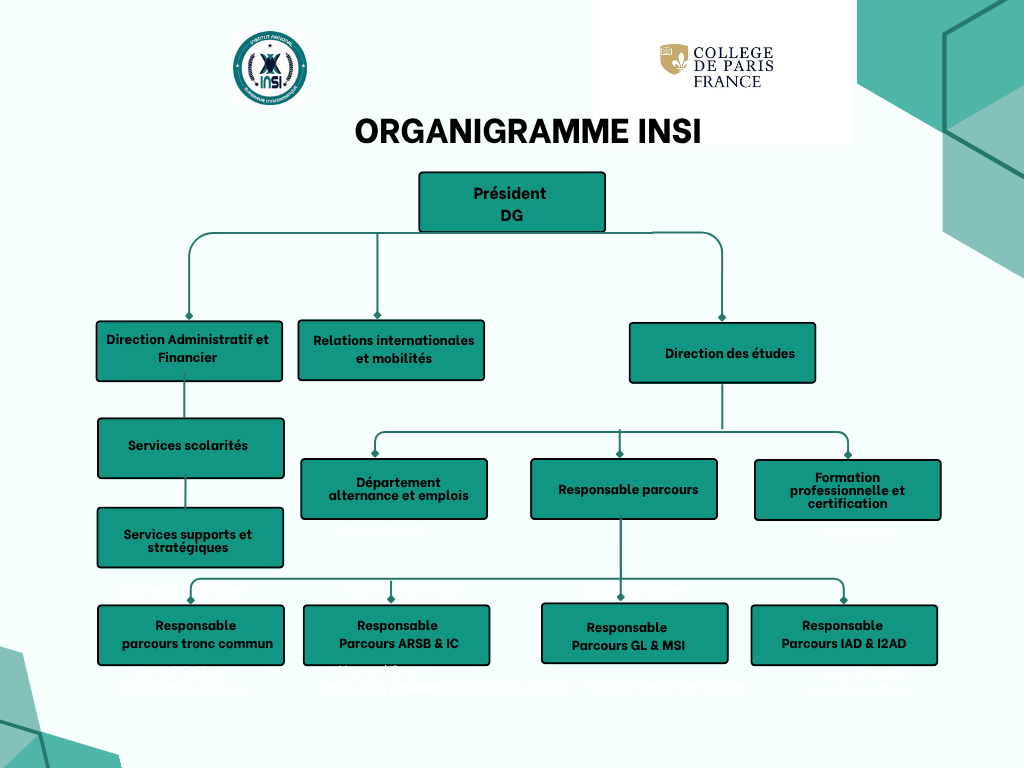
\includegraphics[width=6.89375in,height=5.86389in]{../figures/image1.png}

\textbf{Figure 1~: Organigramme de l'INSI}

L\textquotesingle organigramme de l'INSI, en partenariat avec le Collège
de Paris, est structuré autour d'une direction générale incarnée par le
Président Directeur Général. Ce dernier assure la coordination de trois
pôles principaux : la Direction Administrative et Financière, la
Direction des Études, et le service des Relations Internationales et
Mobilités.

Le Président Directeur Général assure la direction
stratégique de l'institut. Il supervise l'ensemble des activités
pédagogiques, administratives et de développement.

Il veille à la qualité de l'enseignement, à la bonne gestion des
ressources humaines et matérielles, et représente l'établissement auprès
des partenaires et autorités.

La Direction Administrative et Financière est chargée de la
gestion des affaires internes, notamment à travers deux services
essentiels : le service des scolarités, qui s'occupe des
dossiers étudiants, inscriptions et suivi académique, et les
services supports et stratégiques, qui assurent un appui
logistique, administratif et technologique à l'ensemble de l'institut.

Le pôle des Relations Internationales et Mobilités gère les
échanges académiques avec l'étranger ainsi que les projets de mobilité
étudiante ou enseignante.

La Direction des Études supervise quant à elle l'ensemble des
programmes pédagogiques et le corps enseignant. Elle travaille en
étroite collaboration avec un Responsable Parcours, qui
coordonne les différentes spécialisations proposées. Cette direction
intègre également une cellule dédiée à la formation
	professionnelle et à la certification, en charge des dispositifs de
validation des compétences, des certifications professionnelles et des
parcours de formation continue. Il comprend également le
Département alternance et emplois, responsable du suivi des
étudiants en contrat d'alternance, des stages professionnels, et de
l'insertion professionnelle.

Sous la partie Responsable Parcours, plusieurs responsables
pédagogiques gèrent les différentes filières de formation : le
parcours tronc commun, qui regroupe les matières fondamentales
partagées par tous les étudiants en début de cycle ; le parcours
	ARSB \& IC; le parcours GL \& MSI ; et enfin le
parcours IAD \& I2AD.

D'autres structures, bien que non représentés sur cet organigramme,
contribuent également de manière significative à la mission de l'INSI.

Le Conseil de l'École, Il regroupe des membres de l'équipe
pédagogique et administrative. Il joue un rôle consultatif ou
décisionnel sur les questions académiques : validation des programmes,
suivi des résultats, discipline, méthodologie, etc.

Le responsable de la formation en ligne, Il conçoit et
supervise les dispositifs d'apprentissage à distance. Il s'assure que
les contenus en ligne sont accessibles, interactifs et conformes aux
standards pédagogiques, tout en accompagnant enseignants et étudiants
dans leur utilisation.

L'Association et Clubs étudiants, encadre et soutient les
initiatives étudiantes, les clubs thématiques (informatique, innovation,
sport, culture, etc.), et les événements organisés dans le cadre de la
vie étudiante. Cela favorise l'engagement, le développement personnel et
les compétences transversales des étudiants.

Cette structure témoigne d'une organisation à la fois pédagogique,
administrative et tournée vers l'international et l'employabilité,
assurant une formation complète et professionnalisante aux étudiants.

\begin{enumerate}
	\def\labelenumi{\arabic{enumi}.}
	\setcounter{enumi}{1}
	\item
	\textbf{Domaine de spécialisation}
\end{enumerate}

INSI University propose des parcours académiques
	professionnalisants dans le domaine de l'informatique et des
technologies numériques, articulés autour de licences professionnelles,
de masters spécialisés, formations professionnelles continues et
d'opportunités de mobilité internationale.

\begin{enumerate}
	\def\labelenumi{\alph{enumi})}
	\item
	\textbf{\uline{Licences professionnelles}}
\end{enumerate}

Les programmes de licence offrent une formation de base solide, axée sur
la pratique, et préparant à une insertion rapide dans le monde
professionnel :

GL (Génie Logiciel) : Conception, développement et maintenance
d\textquotesingle applications logicielles.

ARSB (Administration Réseaux et Systèmes et Base de données) :
Gestion d'infrastructures informatiques, réseaux, serveurs et systèmes.

IAD (Intelligence Artificielle et Data Science) : Introduction
aux algorithmes d'IA, au traitement de données et à l'apprentissage
automatique.

\begin{enumerate}
	\def\labelenumi{\alph{enumi})}
	\setcounter{enumi}{1}
	\item
	\textbf{\uline{Masters professionnels}}
\end{enumerate}

Les masters permettent d'approfondir les compétences techniques et
managériales, en lien étroit avec les évolutions du secteur :

MSI (Management des Systèmes d'Information) : Pilotage de
projets numériques, gouvernance des SI.

IC (Infrastructures et Cybersécurités) : Sécurisation des
systèmes, audit, réseaux avancés.

IAD (Intelligence Artificielle, Analyse de Données et
	Automatisation) : Applications avancées de l'IA, automatisation des
processus et science des données.

\begin{enumerate}
	\def\labelenumi{\alph{enumi})}
	\setcounter{enumi}{2}
	\item
	\textbf{Formations professionnelles}
\end{enumerate}

INSI University propose également des formations professionnelles
continues, spécifiquement conçues pour les professionnels déjà en poste
souhaitant approfondir leurs compétences ou se spécialiser dans l'un des
domaines proposés.\\
Ces formations sont adaptées aux contraintes des professionnels
(horaires flexibles, modules pratiques) et visent à renforcer leur
employabilité ou à accompagner leur évolution de carrière.

\begin{enumerate}
	\def\labelenumi{\alph{enumi})}
	\setcounter{enumi}{3}
	\item
	\textbf{Mobilité internationale \& double diplôme}
\end{enumerate}

Dans une optique d'ouverture et de reconnaissance internationale, INSI
propose à ses étudiants des opportunités de mobilité académique et de
double diplôme, à partir de la deuxième année (L2).

\begin{itemize}
	\item
	\textbf{Format hybride} : \emph{6 mois de formation à Madagascar + 6
		mois à l'étranger} selon le parcours choisi.
\end{itemize}

\begin{itemize}
	\item
	\textbf{Double diplôme en L3 ou M2} : En partenariat avec des
	institutions internationales telles que :
	
	\begin{itemize}
		\item
		Collège de Paris (France)
	\end{itemize}
	
	\begin{itemize}
		\item
		Keyce Informatique (France)
	\end{itemize}
	
	\begin{itemize}
		\item
		Eskills (Québec, Canada)
	\end{itemize}
\end{itemize}

\hypertarget{conditions-duxe9ligibilituxe9}{%
	\paragraph{\texorpdfstring{\textbf{Conditions
				d'éligibilité}}{Conditions d'éligibilité}}\label{conditions-duxe9ligibilituxe9}}

\begin{itemize}
	\item
	Niveau DALF C1 en français pour la mobilité vers des pays
	francophones.
	\item
	Niveau B2 ou C1 en anglais pour les destinations anglophones.
	
	\begin{enumerate}
		\def\labelenumi{\arabic{enumi}.}
		\item
		Architectures des formations pédagogiques
	\end{enumerate}
\end{itemize}

Le recrutement des étudiants à l'INSI s'effectue exclusivement par
sélection de dossiers pour l'entrée en première année de Licence (L1),
et par voie de concours pour l'admission en Master 1,

Au sein de l'INSI, une seule mention est proposée : Informatique,
déclinée en trois parcours distincts aux niveaux Licence et Master :

Tableau 1~: Les parcours en Licence et Master

\begin{table}[H]
	\centering
	\begin{tabular}{|p{7cm}|p{7cm}|}
		\hline
		\textbf{Licence} & \textbf{Master} \\
		\hline
		Génie Logiciel (GL) & Management des Systèmes d’Information (MSI) \\
		\hline
		Administration Réseaux, Systèmes et Bases de données (ARSB) & Infrastructures et Cybersécurités (IC) \\
		\hline
		Intelligence Artificielle et Data Science (IAD) & Intelligence Artificielle, Analyse de Données et Automatisation (I2AD) \\
		\hline
	\end{tabular}
	\caption{Exemple de parcours Licence/Master}
\end{table}


L'architecture des études à trois niveaux conformément au système LMD
(Licence Master et Doctorat) permet les comparaisons et les équivalences
académiques des diplômes au niveau international.

L = Licence (Bac + 3) = L1, L2, L3 = 6 semestres S1 à S6

M = Master (Bac + 5) = M1, M2 = 4 \textbf{semestres S7 à S10}

Le diplôme de licence est obtenu en 3 années des études après
Baccalauréat. Et le

diplôme de Master est obtenu en 2 ans après obtenu du diplôme de
LICENCE.

Le MASTER PROFESSIONNEL est un diplôme destiné à la recherche emploi au
terme

des études.

\textbf{Spécificités pédagogiques}

\begin{itemize}
	\item
	\textbf{École d\textquotesingle alternance dès la L2 S4}\\
	Alternance cours/entreprise pour une meilleure insertion
	\item
	\textbf{Écoles connectées \& e-learning}\\
	Plateforme numérique de formation, cloud intégré, Google Workspace\\
	Cours accessibles en ligne selon les parcours
	\item
	\textbf{Pédagogie active \& par projets\\
		Hackathons, soutenances exposées, projets réels en entreprise}
	
	\begin{enumerate}
		\def\labelenumi{\arabic{enumi}.}
		\item
		\textbf{Relations de l'INSI avec les entreprises et les organismes}
	\end{enumerate}
\end{itemize}

L'Institut National Supérieur en Informatique (INSI) entretient des
liens étroits avec le monde professionnel. L'INSI collabore activement
avec de nombreux organismes publics, semi-publics et privés, tant au
niveau national qu'international. Cette collaboration se traduit
concrètement par l'organisation régulière de stages obligatoires pour
les étudiants, favorisant leur immersion professionnelle et leur
employabilité.

Parmi les entreprises et institutions partenaires accueillant nos
étudiants en stage chaque année, on peut citer : Data Pulse Center,
RELIA Consulting, Code Talent, Bocasay, Minimad, Smartone AI, NOVITY,
Eclosia Madagascar, VISEO Groupe, Océane Trade, ACCES Banque, ...

En plus des stages, l'INSI organise régulièrement des visites
	pédagogiques, des rencontres métiers et des projets
	collaboratifs avec plusieurs entreprises du secteur technologique et
numérique. Ces activités permettent aux étudiants de mieux comprendre
les réalités du terrain, d'échanger avec des professionnels et de
s'ouvrir à l'environnement entrepreneurial.

Parmi les entreprises ayant accueilli ces initiatives : NOVITY, YAS
Madagascar, Smartone AI, Eclosia Madagascar, et d\textquotesingle autres
acteurs majeurs du numérique à Madagascar.

Cette dynamique de partenariat permanent constitue un pilier de la
pédagogie à l'INSI, en lien avec son objectif de former des
professionnels compétents, opérationnels et ancrés dans les besoins du
marché.

\begin{enumerate}
	\def\labelenumi{\arabic{enumi}.}
	\setcounter{enumi}{1}
	\item
	\textbf{Partenariat au niveau international}
\end{enumerate}

L'INSI s'est inscrit dans une dynamique d'ouverture à l'international
grâce à son partenaire fondateur, ILO Madagascar, représentant
de l'Organisation Internationale du Travail. Cette orientation se
renforce aujourd'hui à travers des partenariats stratégiques
	avec des institutions académiques et des entreprises internationales,
permettant à l'Institut de proposer une formation alignée sur les
standards mondiaux.

L'INSI bénéficie actuellement de programmes de co-diplomation et
	de double diplôme en collaboration avec plusieurs établissements
internationaux de renom, tels que :

\begin{itemize}
	\item
	\textbf{Collège de Paris International}
	\item
	\textbf{Keyce Informatique} (France)
	\item
	\textbf{Eskills Academy} (Québec, Canada)
	\item
	\textbf{École Supérieure Polytechnique d'Antsiranana (ESPA)} -- pour
	une synergie régionale renforcée.
\end{itemize}

Ces partenariats permettent non seulement d'enrichir l'offre
pédagogique, mais aussi d'ouvrir des perspectives de mobilité
	académique et professionnelle aux étudiants, en leur offrant
une reconnaissance de leurs compétences à l'échelle internationale.

Par ailleurs, à travers les stages annuels et projets
	pédagogiques, l'INSI collabore également avec des entreprises à
dimension régionale ou mondiale, telles que :

\begin{itemize}
	\item
	\textbf{VISEO Groupe}
	\item
	\textbf{Eclosia Madagascar} (Groupe mauricien)
	\item
	\textbf{Smartone AI}
	\item
	\textbf{NOVITY}, entre autres.
\end{itemize}

Ces relations actives témoignent de l'ancrage de l'INSI dans un
écosystème global, plaçant l'Institut comme un acteur majeur de
la formation en informatique à Madagascar, tourné vers l'innovation et
les exigences du marché international.

\begin{enumerate}
	\def\labelenumi{\arabic{enumi}.}
	\item
	\textbf{Parcours professionnels des diplômés}
\end{enumerate}

Les diplômés de la Licence en Informatique de l'INSI disposent d'un
socle solide de compétences en programmation, systèmes, réseaux, bases
de données et développement logiciel. Cette polyvalence leur permet
d'intégrer directement le marché du travail ou de poursuivre en Master.
À ce niveau, ils peuvent exercer en tant que :

\begin{itemize}
	\item
	\textbf{Technicien système et réseau}
	\item
	\textbf{Développeur web / mobile (front-end ou back-end)}
	\item
	\textbf{Administrateur systèmes junior}
	\item
	\textbf{Technicien support IT}
	\item
	\textbf{Intégrateur / testeur logiciel}
	\item
	\textbf{Assistant en sécurité informatique}
	\item
	\textbf{Assistant en projets d'IA ou de data (selon profil)}
\end{itemize}

Les stages annuels en entreprise leur offrent une première expérience
professionnelle valorisante dans des structures variées : entreprises
technologiques, banques, administrations, startups, ONG, etc.

La formation de Master proposée à l'INSI, grâce à ses parcours
spécialisés, forme des professionnels capables d'intervenir sur des
projets complexes, innovants et à dimension stratégique. Les débouchés
varient selon la spécialisation choisie :

\hypertarget{parcours-inguxe9nierie-logicielle-ruxe9seaux-et-systuxe8mes}{%
	\subparagraph{Parcours Ingénierie logicielle, réseaux et systèmes
		:}\label{parcours-inguxe9nierie-logicielle-ruxe9seaux-et-systuxe8mes}}

\begin{itemize}
	\item
	\textbf{Ingénieur en développement logiciel / full-stack}
	\item
	\textbf{Architecte logiciel}
	\item
	\textbf{Ingénieur systèmes et réseaux}
	\item
	\textbf{Administrateur cloud / DevOps}
	\item
	\textbf{Chef de projet informatique}
\end{itemize}

\hypertarget{parcours-cybersuxe9curituxe9}{%
	\subparagraph{Parcours Cybersécurité
		:}\label{parcours-cybersuxe9curituxe9}}

\begin{itemize}
	\item
	\textbf{Expert en sécurité des systèmes d\textquotesingle information}
	\item
	\textbf{Analyste SOC / CERT}
	\item
	\textbf{Auditeur en cybersécurité}
	\item
	\textbf{Responsable de la sécurité IT (RSSI)}
\end{itemize}

\hypertarget{parcours-intelligence-artificielle-et-data}{%
	\subparagraph{Parcours Intelligence Artificielle et Data
		:}\label{parcours-intelligence-artificielle-et-data}}

\begin{itemize}
	\item
	\textbf{Data Scientist}
	\item
	\textbf{Data Analyst}
	\item
	\textbf{Ingénieur en Intelligence Artificielle}
	\item
	\textbf{Machine Learning Engineer}
	\item
	\textbf{Développeur d\textquotesingle applications intelligentes}
	\item
	\textbf{Consultant en IA}
	\item
	\textbf{Spécialiste en traitement automatique du langage naturel
		(TALN)}
	\item
	\textbf{Spécialiste en vision par ordinateur (Computer Vision)}
\end{itemize}

Grâce aux partenariats internationaux et aux projets en
	entreprise, les diplômés du Master peuvent également prétendre à des
postes dans des structures multinationales, ou poursuivre une
carrière académique et de recherche (doctorat, enseignement
supérieur).

\begin{enumerate}
	\def\labelenumi{\arabic{enumi}.}
	\item
	\textbf{Ressources humaines}
\end{enumerate}

L'INSI s'appuie sur une équipe pédagogique et administrative compétente,
dynamique et engagée dans la réussite de ses étudiants. Ses ressources
humaines se répartissent comme suit :

Président Directeur de l'INSI~: Dr RAMASONDRANO Andriamanjaka

Responsable parcours~ARSB \& IC~: Mr RATIANARISON Hery Mampionona

Responsable parcours tronc commun : Dr RAKOTONDRAMANANA R, Sitraka

Responsable parcours GL \& MSI~: Mr ANDRIAMIADANA TANTELY ANTOINE

Responsable parcours IAD \& I2AD~: par intérim PDG

Nombres des enseignants : 40

Nombres des personnels administratives : 04

Personnels d'appui~: 6

